\documentclass[paper=a4, fontsize=11pt]{scrartcl}

\usepackage[T1]{fontenc} 
\usepackage{fourier}
\usepackage[spanish]{babel} 
\usepackage[utf8]{inputenc}
\usepackage{amsmath,amsfonts,amsthm}  
\usepackage{graphicx}
\usepackage{hyperref}

\usepackage{sectsty}
\usepackage{xcolor}
\definecolor{sectioncolor}{rgb}{0.2, 0.2, 0.6}
\allsectionsfont{\color{sectioncolor}\centering \normalfont\scshape} 

\numberwithin{equation}{section}
\numberwithin{figure}{section} 
\numberwithin{table}{section} 

\setlength\parindent{0pt}

\newcommand{\horrule}[1]{\rule{\linewidth}{#1}} 

\setcounter{tocdepth}{1}


\hypersetup{
    colorlinks=true,       % false: boxed links; true: colored links
    linkcolor=sectioncolor,          % color of internal links (change box color with linkbordercolor)
    citecolor=sectioncolor,        % color of links to bibliography
    filecolor=sectioncolor,      % color of file links
    urlcolor=sectioncolor           % color of external links
}



\title{	
\normalfont \normalsize 
\textsc{Curso 2014/2015} \\ [25pt] 
\horrule{2pt} \\[0.5cm] 
\huge Variable Compleja I\\ 
\horrule{2pt} \\[0.5cm] 
}

\author{Guillermo Ruiz Álvarez} 

\date{\normalsize\today}

\AtBeginDocument{
  \addtocontents{toc}{\small}
}

\begin{document}

\maketitle 

Me he dedicado a ir escribiendo cosas de Variable Compleja a medida que he ido leyendo apuntes y haciendo los ejercicios. Aquí hay cero formalismos así que no me peguéis si os chirría algo. Para comprender la asignatura mirad los apuntes de Pedro. Esto es para repasar y tener una visión general de todo (teoremas, resultados, cosas en general). Seguramente haya mil errores, así que sentíos libres de añadir/quitar lo que queráis. Si veis que falta algo y no os apetece cambiar el \texttt{.tex} decidlo a cualquiera nosotros.

Como son veinte páginas no me he atrevido a titularlo resumen.
\pagenumbering{gobble}
\begin{flushright}
\textit{Con hamor}

\textit{Rual}
\end{flushright}

\tableofcontents

\newpage
\pagenumbering{arabic}
\section{Números complejos}
Definimos $i$ como sigue: $\boxed{i^2=-1}$ y partimos de
\begin{equation*}
\left\{
\begin{array}{l l}
z=x+iy & \text{Número complejo}\\
\overline{z}=x-iy & \text{Conjugado de } $z$
\end{array}
\right.
\end{equation*}
con $x,y \in \mathbb{R}$

\subsection{Propiedades}

\subsubsection{Propiedades generales}\mbox{}

\begin{itemize}
\item $\Re(z)=x=\frac{1}{2}(z+\overline{z})$
\item $\Im(z)=y=\frac{1}{2i}(z-\overline{z})$
\item $|z|=\sqrt{x^2+y^2}$
\item $|z|^2=z\cdot\overline{z}$
\item $\frac{1}{z}=\frac{\overline{z}}{|z|^2}$
\item $|z+w|\le|z|+|w|$
\end{itemize}

\subsubsection{Identidades del conjugado}\mbox{}
\begin{itemize}
\item $\overline{z+w} = \overline{z}+\overline{w}$
\item $\overline{z\cdot w} = \overline{z}\cdot \overline{w}$
\item $\overline{\frac{z}{w}} = \frac{\overline{z}}{\overline{w}}$
\item $\overline{z^n}=\overline{z}^n$\hspace{5mm}$n\in\mathbb{Z}$
\item $|\overline{z}| = |z|$
\item $\overline{e^z} = e^{\overline{z}}$
\end{itemize}

\subsection{Representación}

\subsubsection{Representación polar}\mbox{}

Un número complejo $z=x+iy$ se puede representar en un plano (el plano complejo) como un vector de coordenadas $\Re(z)$ y $\Im(z)$.

\begin{itemize}
\item El módulo del vector sería el módulo del número complejo $\boxed{|z|=\sqrt{x^2+y^2}}$
\item El ángulo $\theta$ que forma el vector con el eje $x$ cumple $tan(\theta) = \frac{y}{x}$, luego $\boxed{\theta = tan^{-1}\left(\frac{y}{x}\right)}$
\end{itemize}

\subsubsection{Fórmula de Euler}\mbox{}

$$\boxed{e^{i\theta}=cos(\theta)+i\sin(\theta)}$$
\begin{itemize}
\item El módulo de este número es $|e^{i\theta}|=\sqrt{cos^2(\theta)+sin^2(\theta)} = 1$
\end{itemize}

Por tanto
\begin{itemize}
\item Cualquier número complejo se puede expresar como $\boxed{z=|z|e^{i\theta}}$, con $\theta\in\mathbb{R}$.
\item De esta forma $|z|=|z|\cdot|e^{i\theta}|=|z|\cdot 1=|z|$
\item El ángulo que forma con el eje x es $\theta$, ya que $\theta = \tan^{-1}\left(\frac{sin(\theta)}{cos(\theta)}\right)=\tan^{-1}(tan(\theta))$.
\end{itemize}

\paragraph{Propiedades}
Sean $z,w\in\mathbb{C}$ y sea $z=x+iy$ con $x,y\in\mathbb{R}$
\begin{itemize}
\item $e^z = e^{x+iy} = e^x\cdot e^{iy}$
\item $e^{z}\cdot e^{w}=e^{z+w}$
\end{itemize}

\newpage
\subsubsection{Esfera de Riemann}\mbox{}
\label{sec:riemann}

Mediante la proyección estereográfica (\ref{fig:estereo}) podemos llevar la esfera unidad ($\mathbb{S}^2$) en el plano complejo. El único punto que no es proyectable es el $\vec{N}=(0,0,1)$. Se define que su proyección sea $\infty$ de manera que tenemos una biyección entre $\mathbb{S}^2$ y $\hat{\mathbb{C}}=\mathbb{C}\cup\{\infty\}$, que denotaremos como $\pi:\mathbb{S}^2\longrightarrow \mathbb{R}$

\begin{figure}[htbp]
\centering
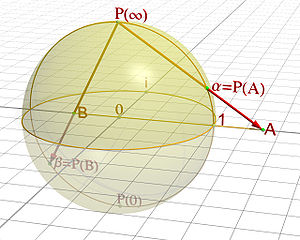
\includegraphics[width=0.5\textwidth]{estereo.jpg}
\caption{Proyección estereográfica}
\label{fig:estereo}
\end{figure}

De esta forma
\begin{itemize}
\item La circunferencia unidad ($\mathbb{S}^1$) queda invariante por la proyección, es decir, los $z$ con $|z|=1$.
\item La parte superior de la esfera se proyecta sobre la parte del plano que corresponde a los $z$ con $|z|>1$. Es decir, a la parte del plano que queda fuera de la circunferencia unidad.
\item La parte inferior de la esfera se proyecta sobre la parte del plano que corresponde a los $z$ con $|z|<1$. Es decir, a la parte del plano que queda dentro de la circunferencia unidad.
\item El polo norte de la esfera se proyecta sobre $\infty$.
\item El polo sur de la esfera se proyecta sobre $0$.
\item La distancia de dos puntos en $\hat{\mathbb{C}}$ es $d(z,w)=|z-w|$.
\item La distancia de dos puntos en $\mathbb{S}^2$ es la distancia entre las inversas de las proyecciones $\hat{d}(z,w)=|\pi^{-1}(z)-\pi^{-1}(w)|$.
\end{itemize}

\newpage
\subsection{Convergencia y continuidad}
Dada la distancia d en $\mathbb{C}$: $d(z,w)=|z-w|$
\begin{itemize}
\item Convergencia: $\boxed{\lim_{n\to\infty}{z_n}=z \iff \forall\varepsilon\exists n_0: d(z,z_n)<\varepsilon \ \forall n>n_0}$
\item Continuidad: $\boxed{f(z)\text{ continua en } z_0 \iff \forall \varepsilon \exists \delta: d(z,z_0)<\delta \implies d(f(z), f(z_0))<\varepsilon}$
\item $\mathbb{C}, \hat{\mathbb{C}}$ y $\mathbb{S}^2$ con sus respectivas distancias son espacios completos. Es decir, que toda sucesión de Cauchy es convergente.
\item Sucesión de Cauchy: $\{z_n\}_{n\in\mathbb{N}}$ es de Cauchy $\iff \forall\varepsilon \exists N: d(z_n,z_m)<\varepsilon\ \forall n,m > N$.
\end{itemize}

\newpage
\section{Funciones holomorfas}
\begin{itemize}
\item $f(z)$ es holomorfa en $z_0$ si existe el límite: $\boxed{f'(z_0) = \lim_{z\to z_0}\frac{f(z)-f(z_0)}{z-z_0}}$
\item $f$ es \textbf{entera} si es holomorfa en todo punto.
\end{itemize}
\subsection{Propiedades}
\begin{itemize}
\item $f$ holomorfa en $z_0$ $\implies f(z)$ es continua en $z_0$.
\item $f,g$ son holomorfas en $z_0$ $\implies f+g,f\cdot g, f/g$ (donde $g$ no se anule) y $f(g(z))$ son holomorfas en $z_0$.
\item $f$ holomorfa en $z_0$ $\implies f'$ holomorfa en $z_0$.
\item $f$ función y $f'=0\implies f$ es constante.
\item $f$ función y $\Re( f)$ es constante $\implies f$ es constante.
\item $f$ función y $\Im( f)$ es constante $\implies f$ es constante.
\item $f$ función y $|f|$ es constante $\implies f$ es constante.
\item \textbf{Teorema de la función inversa:} $f$ holomorfa en $z_0$ y $f'(z_0)\neq 0$ $\implies f$ es localmente biyectiva y la función inversa $f^{-1}$ es localmente holomorfa con derivada $(f^{-1}(z_0))' = (f'(z_0))^{-1}$.
\end{itemize}

\subsection{Ecuaciones de Cauchy-Riemann}
Podemos definir $f(z) = u(x,y)+iv(x,y)$
\begin{itemize}
\item Si $f$ es holomorfa $\implies \boxed{
\left\{
\begin{array}{ll}
u_x=v_y&\text{Ecuaciones de}\\
u_y=-v_x&\text{Cauchy-Riemann}
\end{array}
\right.}$
\item Si $f$ es holomorfa $\implies \Delta u=\Delta v = 0$
\item Si $u, v$ diferenciables y $u,v$ cumplen Cauchy-Riemann $\implies f$ holomorfa.
\end{itemize}

\subsection{Derivada compleja}
Si $f$ es holomorfa, su derivada se calcula de las siguientes formas (todas equivalentes).
\begin{itemize}
\item Si $f$ depende sólo de $z$, entonces $f'(z)$ se calcula derivando respecto a $z$.
\item $f'(z) = u_x + i v_x$
\item $f'(z) = v_y - i u_y$
\item $f'(z) = \partial_zf = \frac{1}{2}(f_x-if_y)$
\end{itemize}
\begin{center}
Si $\left\{\begin{array}{l l}\partial_{\overline{z}} f = \frac{1}{2}(f_x+if_y) = 0\\ u,v \text{ diferenciables}\end{array}\right.$ $\implies$ $f$ es holomorfa.
\end{center}


\section{Series}
Una serie es una suma infinita de número complejos:
$$\sum_{n=0}^\infty z_n = \lim_{N\to\infty} s_N = \lim_{N\to\infty}\sum_{n=0}^N z_n$$
\begin{itemize}
\item Si $s_N$ converge $\implies z_n\to 0$ cuando $n\to \infty$.
\item Si $\sum_{n=0}^N |z_n|$ converge $\implies \sum_{n=0}^N z_n$ converge y se dice que lo hace \textbf{absolutamente}.
\end{itemize}

\subsection{Criterio M de Weierstrass}
Sea $\{f_n\}_{n\in\mathbb{N}}$ una sucesión de funciones compleja
\begin{itemize}
\item Convergencia puntual: $f_n\to_p f \iff \forall \varepsilon \forall z \exists N: d(f_n(z), f(z))<\varepsilon$ si $n>N$.
\item Convergencia uniforme: $f_n\to_u f \iff \forall \varepsilon \exists N \forall z: d(f_n(z), f(z))<\varepsilon$ si $n>N$.
\end{itemize}

Si $|f_n|$ está acotada por $M_n$ para cada $n\in\mathbb{N}$ entonces
$$\sum_{n=0}^\infty M_n \text{ converge} \implies \sum_{n=0}^\infty |f_n| \text{ converge uniformemente}$$


\subsection{Series de potencias}
Una serie de potencias centrada en $z_0$ es una suma infinita de potencias de un número complejo:
$$\sum_{n=0}^\infty a_n(z-z_0)^n = \lim_{N\to\infty}\sum_{n=0}^N a_n(z-z_0)^n$$

\begin{itemize}
\item Si $|z-z_0|<1 \implies \sum_{n=0}^\infty a_n(z-z_0)^n$ converge
\item Si $|z-z_0|>1 \implies \sum_{n=0}^\infty a_n(z-z_0)^n$ diverge
\item Si $|z-z_0|=1$ hay que estudiar cada caso.
\end{itemize}

\textbf{Ejemplo típico:}
Si $|z-z_0|<1$
$$\boxed{\sum_{n=0}^\infty (z-z_0)^n = \frac{1}{1-(z-z_0)}}$$

\subsubsection{Radio de convergencia}
El radio de convergencia indica el tamaño de la bola centrada en $z_0$ donde la serie converge (absoluta y uniformemente).
\begin{itemize}
\item $\boxed{R = \frac{1}{\lim \sup_{n\to \infty} |a_n|^{1/n}}}$
\item Si $a_n\neq 0 \ \forall n \implies \boxed{R = \lim_{n\to\infty}\frac{|a_{n}|}{|a_{n+1}|}}$
\end{itemize}

En sumas y productos, si $A = \sum a_n(z-z_0)^n$ y $B = \sum b_n(z-z_0)^n$ y convergen con radio de convergencia $R_A$ y $R_B$.
\begin{itemize}
\item $\sum_n (a_n+b_n)(z-z_0)^n$ converge con radio de convergencia al menos $\min(R_A, R_B)$.
\item $\sum_n (a_nb_n)(z-z_0)^n$ converge con radio de convergencia al menos $R_AR_B$.
\item $\sum_n \frac{a_n}{b_n}(z-z_0)^n$ converge con radio de convergencia como máximo $\frac{R_A}{R_B}$.
\end{itemize}

\subsection{Producto Cauchy}
$$\left(\sum_n a_n(z-z_0)^n\right)\cdot\left(\sum_n b_n(z-z_0)^n\right) = \sum_n\left(\sum_k a_kb_{n-k}\right)(z-z_0)^n$$

\newpage
\section{Funciones analíticas}
\begin{itemize}
\item Una función $f(z)$ es analítica si para todo $z_0$ existe una serie de potencias $\sum_n a_n(z-z_0)^n$  convergente con radio de convergencia $R$ tal que $\boxed{f(z) =\sum_n a_n(z-z_0)^n\ \ \forall z \in B_R(z_0)}$
\item Si $f(z)=\sum_n a_n(z-z_0)^n$ con radio de convergencia $R \iff f(z)$ es holomorfa en $B_R(z_0)$.
\end{itemize}

\subsection{Principio de ceros aislados}
\begin{itemize}
\item Los puntos donde una función analítica se anula, si existen, son aislados, excepto para la función idénticamente nula $f=0$.
\item \textbf{Aplicación:} Si dos funciones $f,g$ analíticas coinciden en un entorno (es decir, son iguales en un conjunto de puntos no aislados), su diferencia $h=f-g$ también es analítica, y al ser $f,g$ iguales en ese entorno, se tiene que ahí $h=0$. Como $h$ es analítica y los puntos donde se anula no son aislados, sólo puede ser que $h=0$, luego $f=g$ en todo el dominio donde sean analíticas.
\item \textbf{Equivalentemente:} Tenemos una sucesión $\{w_n\}$ que converge a un punto $w$. Si una función analítica cumple $f(w_n) = 0$ para todos los puntos de la sucesión, entonces $f(z)=0$ en todos los puntos donde sea analítica, ya que $w$ es un punto de acumulación.
\item \textbf{¡Cuidado!:} Esto sólo se cumple donde una función sea analítica, si por ejemplo $f$ no es analítica en $w$, tenemos una sucesión $\{w_n\}$ que converge a $w$ y $f(w_n) = 0$ para todos los puntos de la sucesión, entonces $f$ no tiene por qué ser idénticamente cero.
\end{itemize}

\subsection{La función exponencial}
$$f(z) = e^z = \sum_{n=0}^\infty \frac{z^n}{n!}$$

\subsubsection{Propiedades}
\begin{itemize}
\item $f'(z) = e^z$
\item $e^{(z+w)}=e^ze^w$
\item $e^{(x+iy)}=e^x(cos(y)+isin(y))$
\item $(e^z)^n=e^{nz}$
\item $|e^z| = e^x|e^{iy}|=e^x= e^{\Re(z)}$
\item Radio de convergencia $R=\infty$
\end{itemize}

La exponencial transforma las verticales del plano complejo en circunferencias, y las horizontales en rectas (\ref{fig:exp}).
\begin{figure}[htbp]
\centering
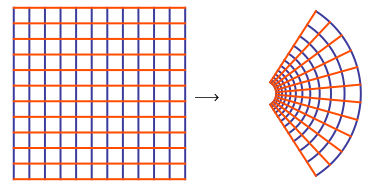
\includegraphics[width=0.5\textwidth]{exp.png}
\caption{$f(z)=e^z$}
\label{fig:exp}
\end{figure}


\subsection{Las funciones trigonométricas e hiperbólicas}
\subsubsection{Funciones trigonométricas}

$$cos(z) = \frac{e^{iz}+e^{-{iz}}}{2} = \sum_{n=0}^\infty(-1)^n\frac{z^{2n}}{(2n)!}$$
$$sin(z) = \frac{e^{iz}-e^{-{iz}}}{2i} = \sum_{n=0}^\infty(-1)^n\frac{z^{2n+1}}{(2n+1)!}$$

\paragraph{Propiedades}
\begin{itemize}
\item $cos'(z) = -sin(z)$
\item $sin'(z) = cos(z)$
\item $sin^2(z)+cos^2(z) = 1$
\item $sin(z\pm w) = sin(z)cos(w)\pm cos(z)sin(w)$
\item $cos(z\pm w) = cos(z)cos(w)\mp sin(z)sin(w)$
\item Radio de convergencia $R=\infty$.
\end{itemize}

\subsubsection{Funciones hiperbólicas}
$$cosh(z) = \frac{e^z+e^{-z}}{2}$$
$$sinh(z) = \frac{e^z-e^{-z}}{2}$$

\subsection{Las funciones logaritmo y raíz}

\subsubsection{La función logaritmo}
El logaritmo complejo es la función inversa de la exponencial compleja, es decir, que \underline{un} logaritmo de $z$ sería \underline{un} $w$ tal que $e^w = z$. Está claro que no se tiene definición en $0$ porque $\nexists z: e^z=0$

El problema a la hora de definir la inversa de la función exponencial es el siguiente, y es que $e^{iz} = e^{iz+i2\pi k}$ $\forall k\in \mathbb{Z}$. Es decir, la exponencial no es inyectiva, los puntos que disten $i2\pi k\ \forall{k}\in \mathbb{Z}$ tienen la misma imagen (\ref{fig:log}). Por tanto, si nos restringimos a cualquier banda horizontal en el plano complejo, la función exponencial es inyectiva sobre ese conjunto de partida.

Se define el logaritmo de un número complejo como
$$\boxed{Log(z) = log(|z|)+i(Arg(z)+2\pi k)}$$
Para cada valor de $k$, se dice que se tiene una \textbf{rama} del logaritmo, siendo $k=0$ la rama principal, es decir, que se ha escogido la banda horizontal $\{z\in\mathbb{C}: -\pi < \Im (z) < \pi\}$

\begin{figure}[htbp]
\centering
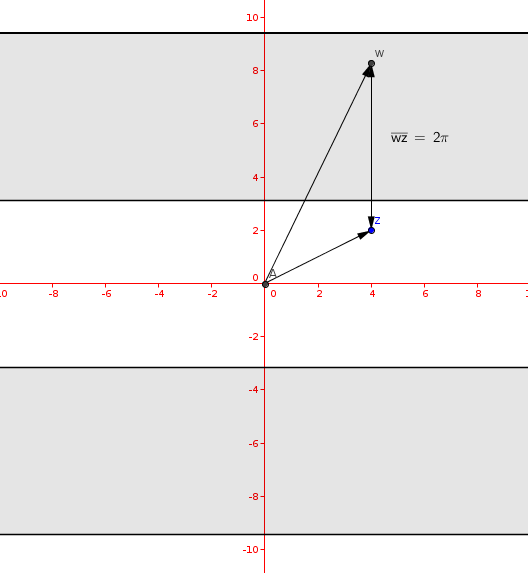
\includegraphics[width=0.5\textwidth]{log.png}
\caption{Función exponencial: puntos con la misma imagen.}
\label{fig:log}
\end{figure}

\paragraph{Cortes de ramificaciones}
Si tomamos la rama principal del logaritmo nos estamos restringiendo, al tomar la exponencial, a la banda horizontal $\{z\in\mathbb{C}: -\pi < \Im (z) < \pi\}$. Si nos fijamos bien, la imagen de todo este conjunto es el plano complejo excepto el radio $\{z\in\mathbb{C}: \Re(z)<0\}$. Esto se puede generalizar para ver que ninguna ramificación del logaritmo puede tomar como conjunto de partida un conjunto donde exista una curva cerrada que tenga índice alrededor de cero, es decir, que rodee al cero.

\subsubsection{La función raíz}
La función raíz es la inversa de la función potencia, es decir, una raíz $n-$ésima de $w$ es $z$ tal que $z^n=w$. En este caso, dado que $w=|w|e^{i(Arg(w)+2\pi k)}$, se tiene que las raíces de $w$ son $\boxed{z=|w|^{\frac{1}{n}}e^{i\left(\frac{Arg(w)+2\pi k}{n}\right)}}$ con $k=0,\hdots,n-1$ siendo $k=0$ la rama principal.

\subsubsection{Raíces de la unidad}
Sabemos que $$1=e^{i2\pi k} = cos(2\pi)+isin(2\pi)\ \forall k\in\mathbb{Z}$$
Las raíces de la unidad son aquellos $z$ tales que $z^n = 1$, es decir $z=\sqrt[n]{1}$.
Tenemos $\boxed{z=e^{i\frac{2k\pi}{n}}}$ tomando $\boxed{k=0,\hdots,n-1}$.

\newpage
\section{Integral compleja}
Si $f(t)=u(t)+iv(t)$
\begin{itemize}
\item $\int_a^b f(t)dt = \int_a^b u(t)dt+i\int_a^b v(t)dt$
\item $\int_a^b cf(t)dt = c\int_a^b f(t)dt$
\item $\left|\int_a^b f(t)dt\right| \le \int_a^b \left|f(t)\right|dt$
\end{itemize}

\subsection{Curvas}
Sea $\gamma$ una curva definida como sigue: $\gamma:[a,b]\to\mathbb{C}$
\begin{itemize}
\item Curva cerrada:  $\gamma(a) = \gamma(b)$
\item Curva simple (sin autointersecciones): $\gamma(a)=\gamma(b) \implies a=b$
\item Curva de Jordan: cerrada y simple.
\item Longitud de una curva: $\int_a^b |d\gamma| = \int_a^b |\gamma'(t)|dt$
\end{itemize}

\subsection{Integral de línea}
$$\int_\gamma f(z)dz = \int_\gamma f(\gamma(t))\gamma'(t)dz$$
Respecto a la longitud de arco tenemos:
$$\int_\gamma f(z)|dz| = \int_\gamma f(\gamma(t))|\gamma'(t)|dt$$
\subsubsection{Propiedades}
\begin{itemize}
\item $\int_\gamma af(z)+bg(z)dz = a\int_\gamma f(z) + b\int_\gamma g(z)$
\item $\gamma = \gamma_1 \circ \gamma_2 \implies \int_\gamma f(z)dz = \int_{\gamma_1} f(z)dz + \int_{\gamma_2} f(z)dz$
\item $\boxed{\left|\int_\gamma f(z)dz\right| \le \int_\gamma |f(z)||dz| \le \sup_{z\in\gamma}\left|f(z)\right|\cdot \int_a^b|\gamma'(t)|dt = \sup_{z\in\gamma}\left|f(z)\right|\cdot long(\gamma)}$
\item Si ${f_n}\to f$ uniformemente $\implies \int f_n \to \int f$ uniformemente.
\end{itemize}

\subsection{Teorema de Green}
$$\int_{\delta\Omega} P \partial x+Q\partial y = \int\int_\Omega \frac{\partial Q}{\partial x} - \frac{\partial P}{\partial y} $$

\subsection{Teorema integral de Cauchy}
$$\text{Si }f(z)\text{ es holomorfa en }\Omega\text{ (dominio simplemente conexo)} \implies \int_{\gamma} f(z)dz = 0.$$ Para todo camino $\gamma\subset\Omega$ cerrado.

\subsection{Teorema integral de Cauchy-Goursat}
Sea $R$ un rectángulo tal que $R\subset\Omega$ simplemente conexo.
$$\text{Si }f(z)\text{ es holomorfa en }\Omega \implies \int_{\delta R} f(z)dz = 0.$$

\subsection{Teoremas}
Sea $\Omega$ un dominio simplemente conexo y $\gamma\subset\gamma$ cualquier camino cerrado.
\begin{itemize}
\item Si $f$ es holomorfa en $\Omega\setminus\{z_i\}$ y $\lim_{z\to z_i} (z-z_i)f(z) = 0 \implies \int_{\gamma}f(z) = 0$.
\item Si $f$ es holomorfa en $\Omega$ $\implies \exists F: F'=f$ en $\Omega$.
\item Si $f:\Omega\to\mathbb{C}\setminus\{0\}$ es holomorfa y $\Omega$ es un dominio simplemente conexo $\implies f$ tiene una rama del logaritmo y una raiz holomorfos.
\item Si $f(z)$ es holomorfa en $\Omega$ y tiene un cero en $z_0$ de multiplicidad $k$, es decir, $f(z_0) = f'(z_0) = \hdots = f^{(n-1)}(z_0) = 0$, entonces $f(z) = (z-z_0)^kg(z)$ siendo $g(z)$ una función holomorfa en $\Omega$.
\end{itemize}

\subsection{Fórmula integral de Cauchy}
\begin{itemize}
\item $Ind_\gamma (z_0) = \frac{1}{2\pi}\left(arg(\gamma(b)-z_0)-arg(\gamma(a)-z_0)\right)$
\item $Ind_\gamma (z_0) = \int_\gamma \frac{dz}{z-z_0}$
\item Es decir, $Ind_\gamma (z_0)$ es el ``número de vueltas que da la curva $\gamma$ al punto $z_0$''.
\end{itemize}
Si $f(z)$ es holomorfa en $B_R(z_0)$
$$\boxed{Ind_\gamma(z_0) f^{(n)}(z_0) = \frac{n!}{2\pi i}\int_\gamma \frac{f(w)}{(w-z_0)^{n+1}}}$$
para todos los puntos $z_0\notin \gamma$.

\subsection{Raíces de una función}
Si $f(z)$ es holomorfa en $\Omega$ y tiene las $n$ raíces $\{{z_i}\}_{i=0,\hdots,n-1}$
$$\sum_{i=0}^n Ind_\gamma(z_i) = \int_\gamma \frac{f'(z)}{f(z)}dz$$
para toda curva cerrada $\gamma\subset\Omega$ que no pase por ninguna raíz.

\subsection{Teorema de Morera}
Sea $\Omega$ un dominio simplemente conexo. Si $f(z)$ cumple $\int_{\gamma} f(z)dz = 0$ para todo camino cerrado $\gamma\subset\Omega$, entonces $f(z)$ es holomorfa en $\Omega$. 

\subsection{Teorema de Liouville}
\begin{itemize}
\item Si $f(z)$ es holomorfa y $|f(z)|<M \implies f$ es constante.
\item Si $f(z)$ es holomorfa y $|f(z)|<a|z|^n + b \implies f$ es un polinomio de grado menor o igual que $n$.
\end{itemize}

\newpage
\section{Series de Laurent}
Una serie de Laurent centrada en $z_0\in\mathbb{C}$ es una serie de la forma
$$\sum_{n=-\infty}^\infty a_n(z-z_0)^n$$

\subsection{Propiedades}
\begin{itemize}
\item Una serie $S$ de Laurent converge si 
$\left\{\begin{array}{l l}
S_{+}=\sum_{n=0}^\infty a_n(z-z_0)^n & \text{ converge}\\
S_{-}=\sum_{n=1}^\infty a_{-n}(z-z_0)^{-n} &  \text{ converge}
\end{array}\right.$
\item Si la serie de converge $\implies S=S_++S_-$
\item El radio de convergencia de $S_+$ es $R = \frac{1}{\lim\sup_{n\to\infty} {|a_n|^{\frac{1}{n}}}}$
\item El radio de convergencia de $S_-$ es $r={\lim\sup_{n\to\infty} {|a_{-n}|^\frac{1}{n}}}$
\item La serie $S$ es convergente en $\left\{z\in\mathbb{C}: r<\left|z-z_0\right|<R\right\}$.
\end{itemize}

Si $f(z)$ es holomorfa en $\left\{z\in\mathbb{C}: r<\left|z-z_0\right|<R\right\}$
entonces
$$f(z) = \sum_{n=-\infty}^\infty a_n(z-z_0)^n$$
y
$$a_n = \frac{1}{2\pi i}\int_{|z-z_0|=\rho} \frac{f(w)}{|w-z_0|^{n+1}}dw$$
con $r<\rho<R$



\newpage
\section{Teorema de los residuos}
\subsection{Singularidad aislada}

Sea $f$ holomorfa en $B_R(z_0)\setminus\{z_0\}$.

\begin{itemize}

\item \textbf{Singularidad evitable: $\lim_{z\to z_0}f(z) = M$}
\item \textbf{Polo:} $\lim_{z\to z_0}|f(z)| = +\infty$
\item \textbf{Singularidad esencial:} $\nexists \lim_{z\to z_0}\left|f(z)\right|$
\end{itemize}

\subsubsection{Singularidad evitable}
\begin{itemize}
\item Si $f$ es holomorfa en $B_R(z_0)\setminus\{z_0\}$ y $\lim_{z\to z_0} (z-z_0)f(z) = 0$, entonces $f(z)$ tiene una singularidad evitable en $z_0$ y

$$ \tilde{f}(z) = 
\left\{
\begin{array}{l l}
f(z) & z\neq z_i\\
M  & z=z_i
\end{array}
\right.$$
es holomorfa en $\Omega$.

\item Todos los coeficientes $a_{-n}$ de la serie de Laurent cumplen $a_{-n}=0$, $n>0$.
\end{itemize}


\subsubsection{Polo}
\begin{itemize}
\item Toda función $f$ con un polo en $z=z_0$ puede representarse como $f(z) = \frac{F(z)}{(z-z_0)^n}$ para un único $n\in \mathbb{Z}$ con $F(z_0)\neq 0$. 

\item Si $n=1$ se dice polo simple (de orden 1). Si $n=2$ se dice polo doble (de orden 2).

\item Si $f(z)$ tiene un polo de orden $n \implies lim_{z\to z_0} (z-z_0)^nf(z) \neq 0, \infty$.

\item Si el polo de $f$ es de orden $m$, los coeficientes de la serie de Laurent cumplen $a_{-m}\neq0$ y $a_{-n}=0$ para $n>m$.
\end{itemize}

\subsubsection{Singularidad esencial}
\begin{itemize}
\item Existen infinitos coeficientes de la serie de Laurent de $f$ que cumplen $a_{-n}\neq 0$ con $n>0$.
\end{itemize}

\subsection{Función meromorfa}
Una función $f(z)$ es meromorfa en $\Omega$ si no tiene singularidades esenciales en $\Omega$. Es decir, es holomorfa en $\Omega\setminus\{z_i\}$ siendo $\{z_i\}$ un conjunto finito, que son los polos de $f(z)$.

\subsection{Residuo}
\begin{itemize}
\item El residuo de una función $f$ holomorfa en $B_R(z_0)\setminus\{z_0\}$ no depende de $\rho\in(0,R)$.
$$\boxed{Res(f(z), z_0) = \frac{1}{2\pi i}\int_{|z-z_0|=\rho} f(z)dz}$$

\item $f(z)$ con $z_0$ una \framebox{\textbf{singularidad evitable}: $R(f(z),z_0) = 0$}
\item $f(z)$ con $z_0$ un \framebox{\textbf{polo simple}: $R(f(z),z_0) = \lim_{z\to z_0} (z-z_0)f(z)$}
\item $f(z)$ con $z_0$ un \framebox{\textbf{polo doble}: $R(f(z),z_0) = \lim_{z\to z_0} \left[(z-z_0)^2f(z)\right]'$}
\item $f(z)$ con $z_0$ un \framebox{\textbf{polo de orden $n$}: $R(f(z),z_0) = \lim_{z\to z_0} \left[(z-z_0)^nf(z)\right]^{(n-1)}$}
\item $f(z)$ con $z_0$ una \framebox{\textbf{singularidad esencial}: $R(f(z),z_0)=a_{-1}$} (siendo $a_{-1}$ el coeficiente de la serie de Laurent).
\end{itemize}

\subsection{Teorema de los residuos}
Sea $\Omega$ un dominio y $\gamma\subset\Omega$ un camino cerrado. Sea $f(z)$ analítica en $\Omega\setminus\{z_i\}$ con $z_i\in\Omega(\gamma)$ (el dominio interior de $\gamma$).

$$\boxed{\sum_i Res\left(f(z), z_i\right)Ind_\gamma(z_i) = \frac{1}{2\pi i}\int_\gamma f(z)dz}$$


\subsection{Cálculo de integrales trigonométricas}
Se puede paramétrizar la circunferencia unidad ($\mathbb{S}^1$) como $z=e^{it}$ con $t\in (0,2\pi)$.
Para los puntos $z$ que estén en $\mathbb{S}^1$ se cumple
$$
\begin{array}{l r}
\boxed{cos(t) = \frac{1}{2}\left(z+\frac{1}{z}\right)} & \boxed{sin(t) = \frac{1}{2i}\left(z+\frac{1}{z}\right)}
\end{array}
$$

$$\boxed{z = cos(t)+isin(t)}$$
\textbf{Nota: } Esto es extensible a circunferencias de radio $R$.
\subsection{Lema de Jordan}
Si $R>0$
$$\boxed{0<\int_0^\pi e^{-Rsin(t)}dt < \frac{\pi}{R}}$$

\begin{itemize}
\item \textbf{Aplicación:} Sobre la circunferencia de radio $R$ parametrizada como $z=Re^{it}$ tomando $t\in (0,2\pi)$ se tiene que
$$\boxed{\left|e^{iz}\right|=e^{-Rsin(t)}}$$
\end{itemize}

\newpage
\section{Teoremas fundamentales de Variable Compleja}

\subsection{Principio del argumento}
Sea $\Omega$ un dominio y $\gamma\subset\Omega$ un camino cerrado que no pasa ni por los polos ni por las raíces de $f(z)$, siendo $f(z)$ una función meromorfa en $\Omega$, con $\{z_i\}$ sus raíces y $\{p_j\}$ sus polos.

$$\sum_i Ind(z_i) - \sum_j Ind(p_j)= \frac{1}{2\pi i}\int_\gamma \frac{f'(z)}{f(z)}$$

Además

$$Ind_{f(\gamma)}(0) = \frac{1}{2\pi i}\int_\gamma \frac{f'(z)}{f(z)}$$

\subsection{Teorema de Rouché}
Sea $\Omega$ un dominio y $\gamma\subset\Omega$ un camino cerrado. Si $f,g$ son funciones holomorfas en $\Omega$ con $|f(z)|>|g(z)|$ sobre $\gamma$, entonces
$$f, f+g \text{ y } f-g \text{ tienen el mismo número de raíces en el dominio que encierra la curva } \gamma.$$

\subsection{Teorema de la aplicación abierta}
Si $f$ es una función holomorfa en un dominio $\Omega$, o $f$ es constante o $f$ es una aplicación abierta (la imagen de un conjunto abierto es un abierto).

\subsection{Principio débil del módulo máximo}
Dado $\Omega$ un dominio acotado y $f$ una función holomorfa en $\Omega$ y continua en $\overline{\Omega}$, entonces el máximo de $|f|$ se alcanza en $\delta\Omega$.

\subsection{Principio fuerte del módulo máximo}
Dado $\Omega$ un dominio y $f$ una función holomorfa en $\Omega$, si $|f|$ alcanza un máximo en $\Omega$, entonces $f$ es constante.

\subsection{Lema de Schwarz}
Sea $f:\mathbb{D}\to\overline{\mathbb{D}}$ holomorfa en $\mathbb{D}=\{z\in\mathbb{C}: |z|<1\}$. Si $\boxed{f(0) = 0}$ \textbf{entonces} $$\boxed{|f(z)|\le|z|}\text{ y }\boxed{|f'(z)| \le 1}$$.

Si $\boxed{|f(z)|=|z|}$ (para $z\neq 0$) o $\boxed{|f'(0)| = 1}$ \textbf{entonces} $$\boxed{f(z) = e^{iy}z}\text{ con }y\in\mathbb{R}$$.

\newpage
\section{Aplicaciones conformes}
Una aplicación conforme es una función $f$ que conserva los ángulos. Si tenemos dos curvas
$$
\begin{array}{l l}
\alpha:[a,b]\to\mathbb{C} & \beta:[a,b]\to\mathbb{C}
\end{array}
$$
entonces
$$arg\left(\frac{\alpha'(t_0)}{\beta'(t_0)}\right) = arg\left(\frac{\left(f\circ \alpha \right)'(t_0)}{\left(f\circ \beta \right)'(t_0)}\right)$$

\textbf{Observación}: Si $f$ es holomorfa y $f'(z_0)\neq 0 \implies f$ es conforme en $z_0$.

\subsection{Teorema de la aplicación conforme de Riemann}
Sea $\Omega$ un dominio simplemente conexo tal que $\Omega\neq\mathbb{C}$. Entonces existe al menos una función $f:\Omega\to\mathbb{D}$ holomorfa y biyectiva.
Si se cumplen las siguientes condiciones, para un $z_0\in\Omega$, entonces dicha función es única.
\begin{itemize}
\item $f(z_0)=0$
\item $f'(z_0)\in\mathbb{R}$
\item $f'(z_0)>0$
\end{itemize}

\subsection{Transformación de Möbius}
Una transformación de Möbius es una función de la forma
$$f(z) = \frac{az+b}{cz+d}$$
con $z,a,b,c,d\in\mathbb{C}$ verificando $ad-bc\neq 0$.
\begin{itemize}
\item Aplicar una transformación de Möbius es realizar una rotación o desplazamiento de la esfera de Riemann (\ref{sec:riemann}) y proyectarla sobre el plano complejo.
\item El punto $-d/c$ se transforma a $\infty$.
\item $\infty$ se transforma a $a/c$.
\item Toda transformación de Möbius lleva circunferencias en $\hat{\mathbb{C}}$ a circunferencias en $\hat{\mathbb{C}}$
\end{itemize}

\subsubsection{Clasificación de transformaciones}
\begin{enumerate}
\item \textbf{Traslación}: $f(z) = z+z_0$
\item \textbf{Dilatación/contracción}: $f(z) = \lambda z$ con $\lambda\in \mathbb{R}$
\item \textbf{Rotación}: $f(z) = e^{yi}z$ con $y\in\mathbb{R}$
\item \textbf{Inversión}: $f(z) = \frac{1}{z}$
\end{enumerate}

\subsubsection{Razón doble}
Dados $z_1,z_2,z_3,z_4\in\mathbb{C}$, se define la razón doble como
$$[z_1,z_2,z_3,z_4] = \frac{(z_1-z_3)(z_2-z_4)}{(z_1-z_4)(z_2-z_3)}$$

\begin{itemize}
\item $T(z) = [z,z_1,z_2,z_3] = \frac{(z-z_2)(z_1-z_3)}{(z-z_3)(z_1-z_2)}$ es una transformación de Möbius que lleva
\begin{itemize}
\item $z_1\to1$
\item $z_2\to0$
\item $z_3\to\infty$
\end{itemize}
y es única.
\item Cualquier transformación de Möbius $f$ cumple
$$[z_1,z_2,z_3,z_4] = \left[f(z_1),f(z_2),f(z_3),f(z_4)\right]$$
\end{itemize}

\end{document}